\documentclass[tikz]{standalone}

\usetikzlibrary{angles, quotes}

\begin{document}
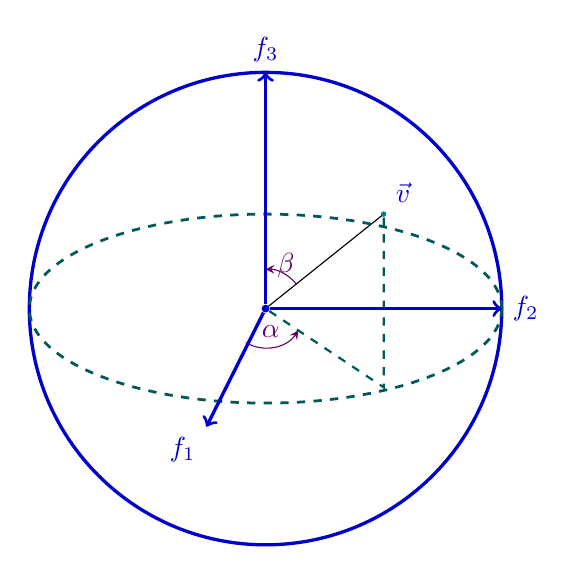
\begin{tikzpicture}

  % Define radius
  \def\r{3}

  % State vector (in CS: data vector)
  \draw (0, 0) node[circle, fill=blue!80!black, inner sep=1] (center) {} 
    -- (\r/2, \r/2.5) node[circle, fill=teal, inner sep=0.7, label=above right:\textcolor{blue!80!black}{$\vec{v}$}] (vect) {};

  \draw[dashed, thick, color=teal!70!black] (center) -- (\r/2, -\r/3) node (anglebase) {} -- (vect);

  % Solid sphere (visualizing memory space)
  \draw[line width=1.2pt, color=blue!80!black] (center) circle (\r);
  \draw[dashed, line width=1pt, color=teal!70!black] (center) ellipse (\r{} and {\r/2.5});

  % Axes (interpreted as feature axes)
  \draw[->, line width=1.2pt, color=blue!80!black] (center) -- ++(-\r/4, -\r/2) node[below left] (feature1) {\textcolor{blue!80!black}{$f_1$}};
  \draw[->, line width=1.2pt, color=blue!80!black] (center) -- ++(\r, 0) node[right] (feature2) {\textcolor{blue!80!black}{$f_2$}};
  \draw[->, line width=1.2pt, color=blue!80!black] (center) -- ++(0, \r) node[above] (feature3) {\textcolor{blue!80!black}{$f_3$}};

  % Angles (interpreted as encoding parameters)
  \pic [draw=violet!80!black, text=violet!80!black, -stealth, "$\alpha$"] {angle = feature1--center--anglebase};
  \pic [draw=violet!80!black, text=violet!80!black, -stealth, "$\beta$", angle eccentricity=1.2] {angle = vect--center--feature3};

\end{tikzpicture}
\end{document}